\documentclass{article}

\usepackage{times}
\usepackage{graphicx} % more modern
\usepackage{natbib}
\usepackage{algorithm, algorithmic}
\usepackage{hyperref}
\usepackage{amssymb, mathtools}
\usepackage{xcolor,colortbl}
\newcommand{\theHalgorithm}{\arabic{algorithm}}
\usepackage{subcaption} % for "subfigure" environment
\usepackage{geometry} 






\usepackage[accepted]{icml2017} 



% The \icmltitle you define below is probably too long as a header.
% Therefore, a short form for the running title is supplied here:
\icmltitlerunning{Globally Induced Forest}

% ============================== CONFIG =================================== %
\graphicspath{{./images/}}
\captionsetup[figure]{size=footnotesize}
% ============================== COLORS =================================== %
\definecolor{orange}{HTML}{FFA500}
\definecolor{dodgerblue}{HTML}{1E90FF}
\definecolor{deepgreen}{HTML}{0AF191}
\definecolor{purplish}{HTML}{E21173}

% ============================== COMMANDS =================================== %
\DeclareMathOperator*{\argmin}{arg\,min}
\DeclareMathOperator*{\argmax}{arg\,max}


\newcommand{\best}{\cellcolor{lightgray}}
\newcommand{\bestA}{\cellcolor{orange}}
\newcommand{\bestB}{\cellcolor{dodgerblue}}


\begin{document} 
\twocolumn[
\icmltitle{Globally Induced Forest: A Prepruning Compression 
Scheme\\Supplementary material}

% It is OKAY to include author information, even for blind
% submissions: the style file will automatically remove it for you
% unless you've provided the [accepted] option to the icml2017
% package.

% list of affiliations. the first argument should be a (short)
% identifier you will use later to specify author affiliations
% Academic affiliations should list Department, University, City, Region, 
%Country
% Industry affiliations should list Company, City, Region, Country

% you can specify symbols, otherwise they are numbered in order
% ideally, you should not use this facility. affiliations will be numbered
% in order of appearance and this is the preferred way.
\icmlsetsymbol{equal}{*}

\begin{icmlauthorlist}
\icmlauthor{Jean-Michel Begon}{ulg}
\icmlauthor{Arnaud Joly}{ulg}
\icmlauthor{Pierre Geurts}{ulg}
\end{icmlauthorlist}

\icmlaffiliation{ulg}{Department of Electrical Engineering and Computer Science
University of Liège, Liège, Belgium}

\icmlcorrespondingauthor{Jean-Michel Begon}{jm.begon@ulg.ac.be}
\icmlcorrespondingauthor{Arnaud Joly}{a.joly@ulg.ac.be}
\icmlcorrespondingauthor{Pierre Geurts}{p.geurts@ulg.ac.be}

% You may provide any keywords that you 
% find helpful for describing your paper; these are used to populate 
% the "keywords" metadata in the PDF but will not be shown in the document

\icmlkeywords{Decision tree, Random forest, Extremely randomized trees, 
pruning, node budget, memory constraint, compression, growing algorithm, greedy 
selection}

\vskip 0.3in
]

\printAffiliationsAndNotice{}




\section{GIF algorithm}
Figure \ref{fig:gif-algo} illustrates visually the inner loop of the GIF 
building algorithm: a subset of the candidates nodes is chosen uniformely at 
random. The contribution of each node is evaluated and the one which reduces 
the error the most is added to the model. Its children are then built and added 
to the candidate list.

\begin{figure*}[ht]    
  \begin{subfigure}[b]{0.5\linewidth}
    \centering
    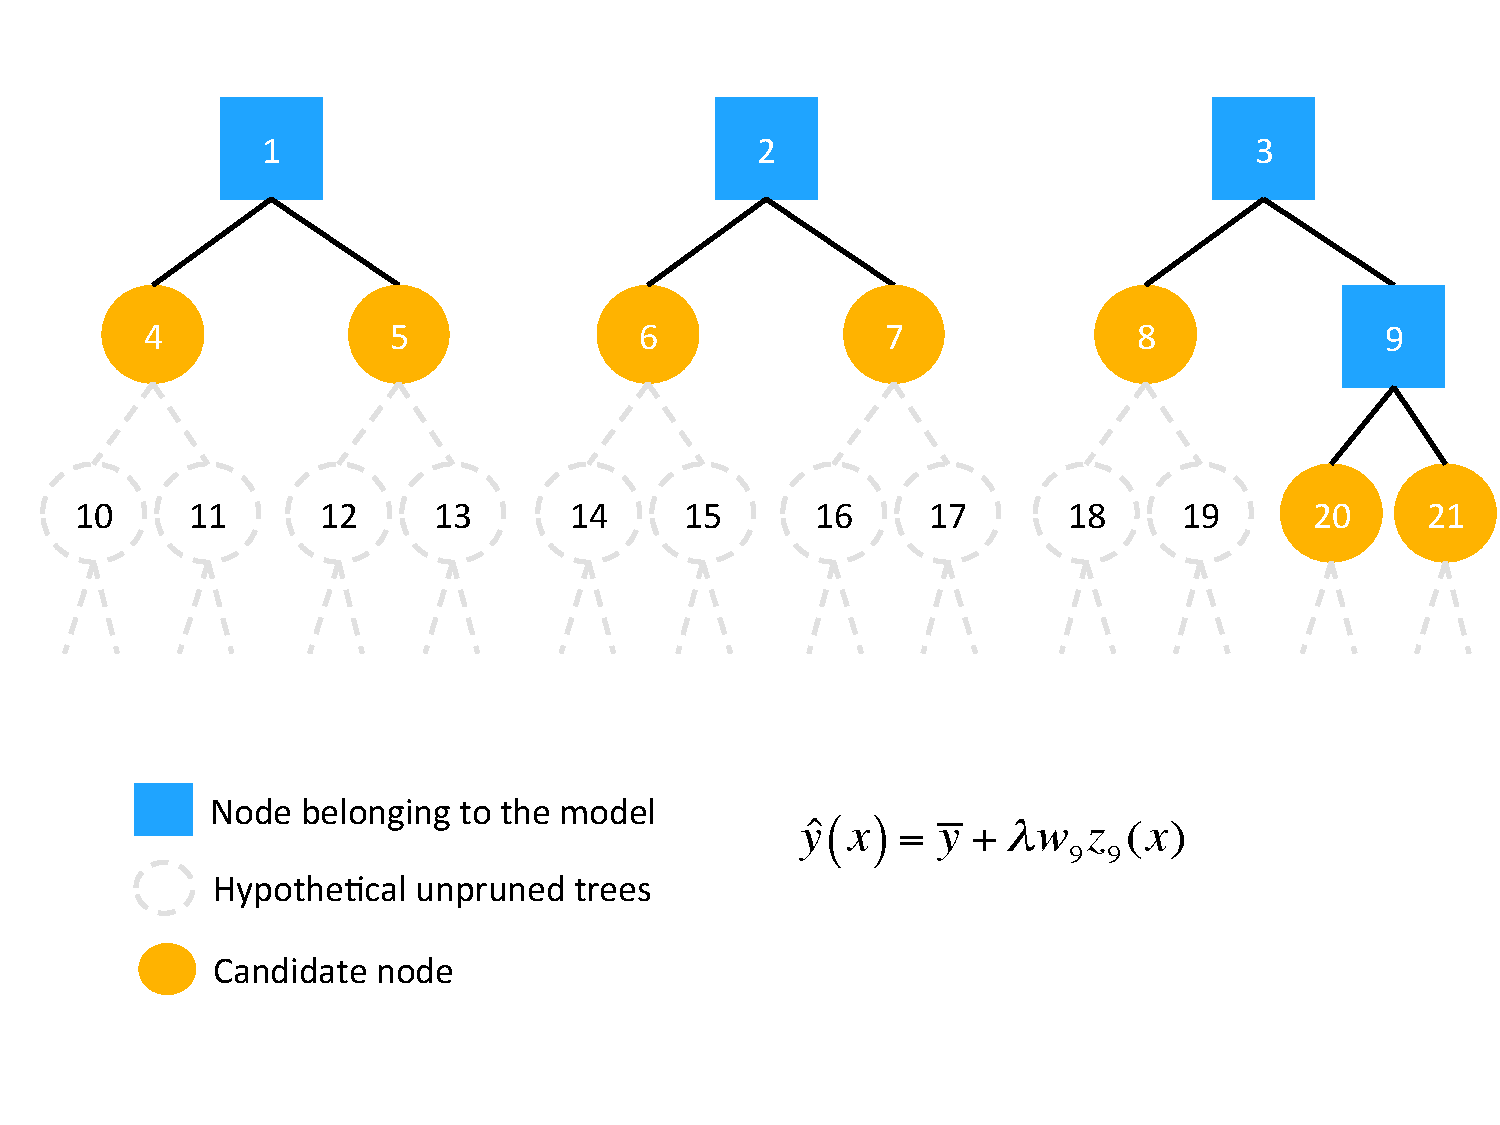
\includegraphics[height=0.25\textheight]{gif_algo1} 
    \caption{Current forest at time $t$} 
    \label{fig:gif-algo1} 
  \end{subfigure} 
  \hspace{\fill}  %% maximize space between adjacent subfigures
  \begin{subfigure}[b]{0.5\linewidth}
    \centering
    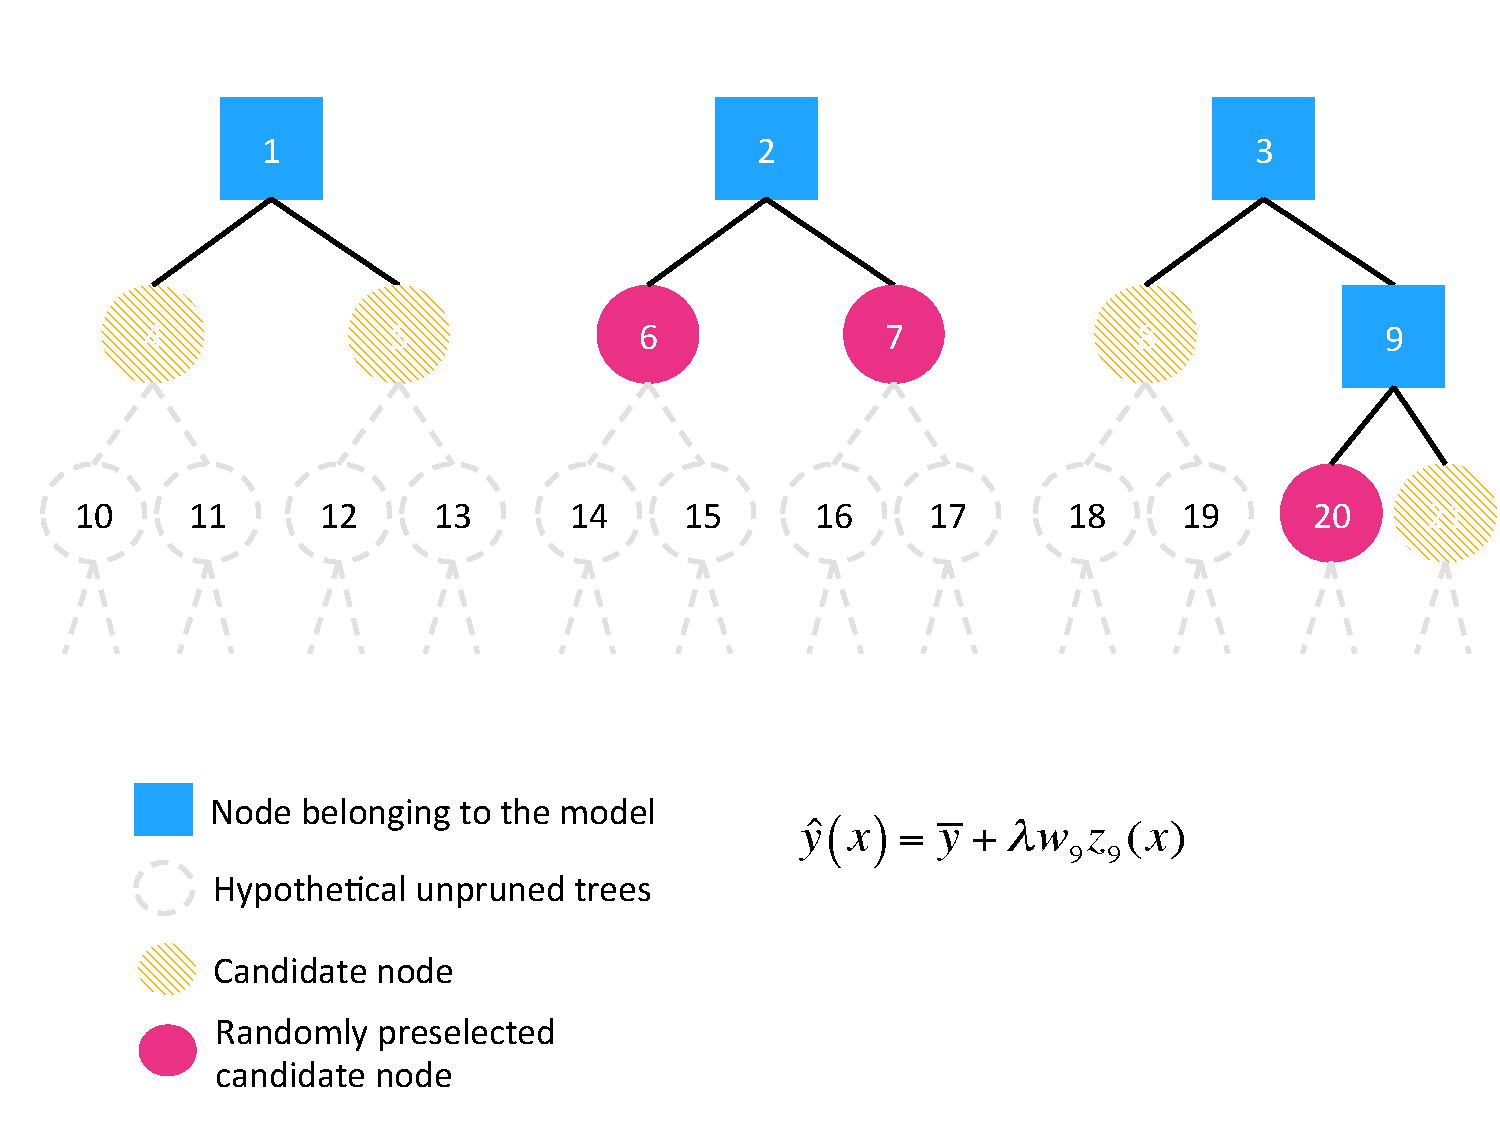
\includegraphics[height=0.25\textheight]{gif_algo2} 
    \caption{A subset of candidates $C_t$  is drawn uniformely at random from 
    the set of candidates $C$ (step 8)} 
    \label{fig:gif-algo2} 
  \end{subfigure} 

  \vspace{4ex}  %% extra vertical space
  \begin{subfigure}[b]{0.5\linewidth}
    \centering
    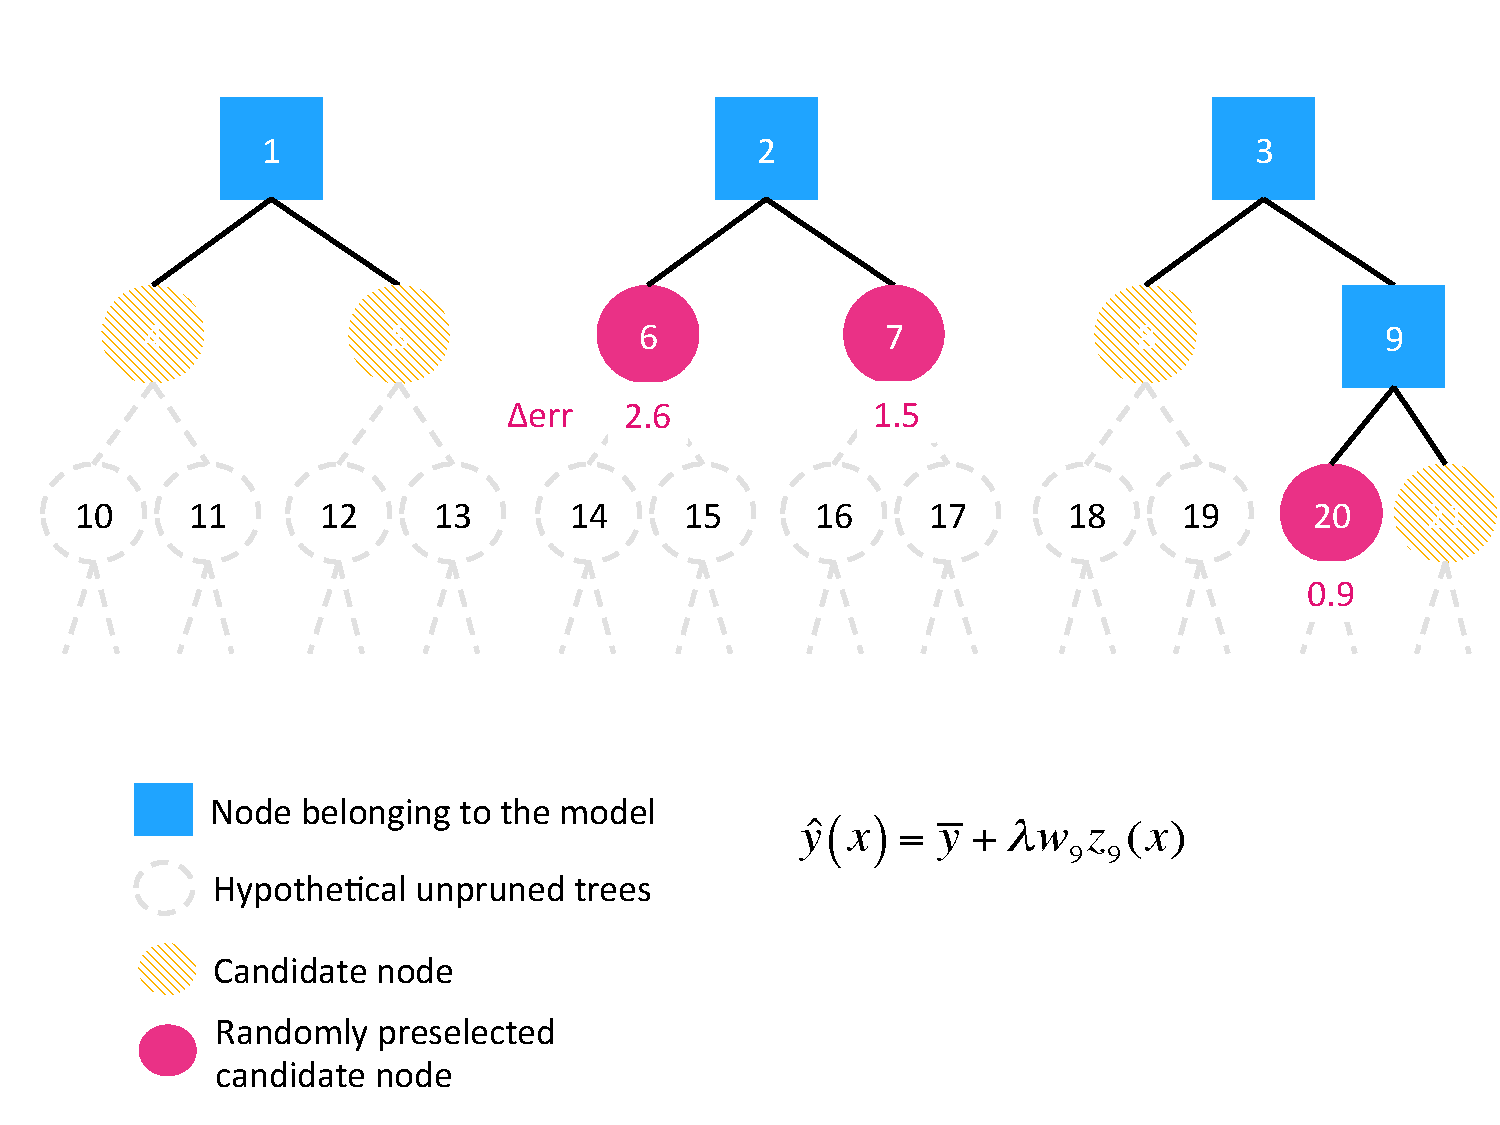
\includegraphics[height=0.25\textheight]{gif_algo3} 
    \caption{The error reduction is computed for all candidates of $C_t$ (step 
    9)} 
    \label{fig:gif-algo3} 
  \end{subfigure} 
  \hspace{\fill}
  \begin{subfigure}[b]{0.5\linewidth}
    \centering
    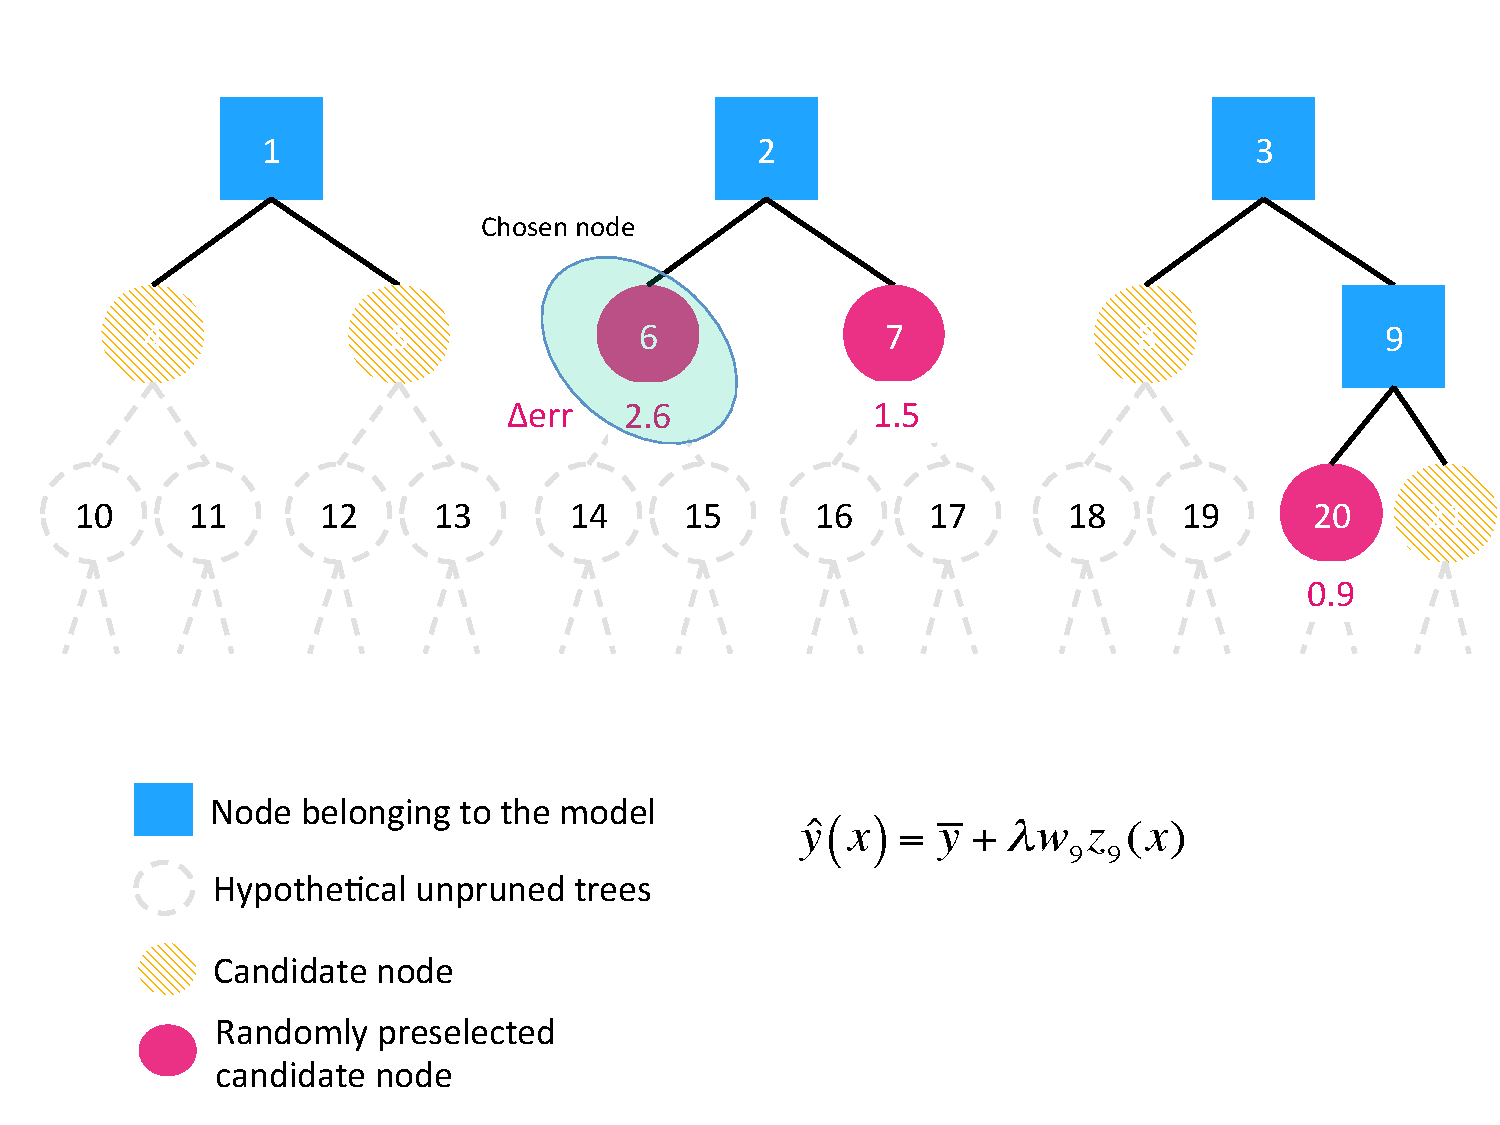
\includegraphics[height=0.25\textheight]{gif_algo4} 
    \caption{The best node (highest error reduction) is selected (step 9)} 
    \label{fig:gif-algo4} 
  \end{subfigure} 

    \vspace{4ex}
  \begin{subfigure}[b]{0.5\linewidth}
    \centering
    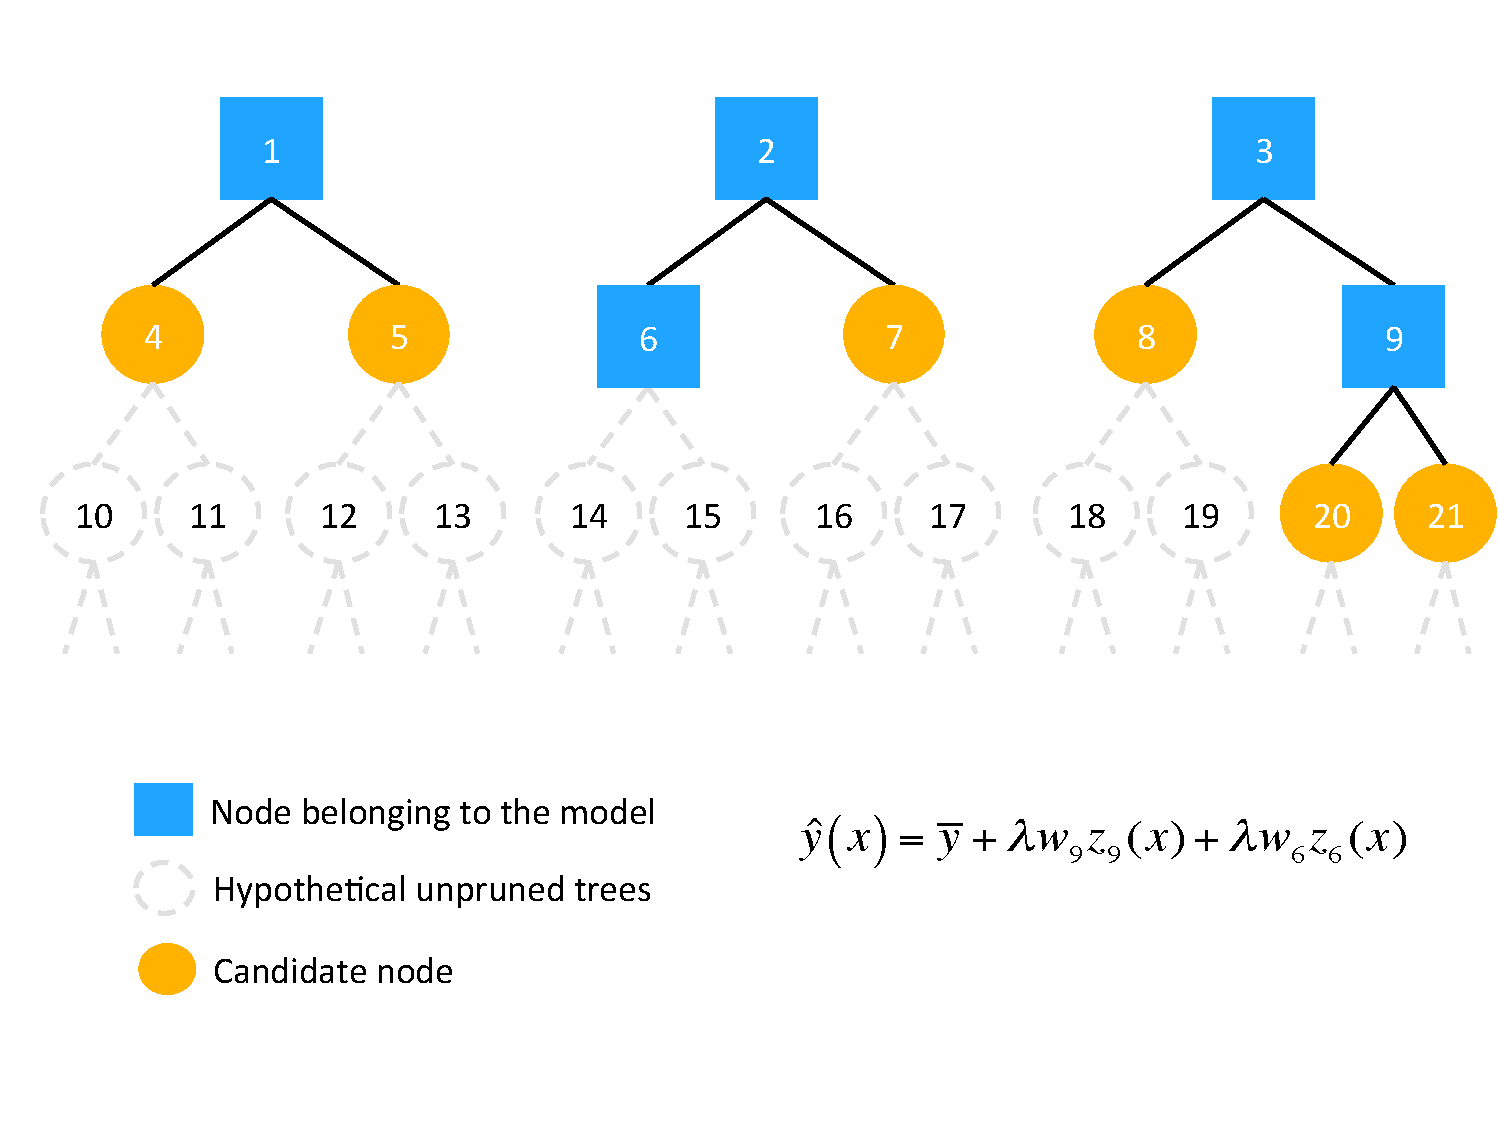
\includegraphics[height=0.25\textheight]{gif_algo5} 
    \caption{The chosen node is introduced in the model (step 10)} 
    \label{fig:gif-algo5} 
  \end{subfigure}
  \hspace{\fill}
  \begin{subfigure}[b]{0.5\linewidth}
    \centering
    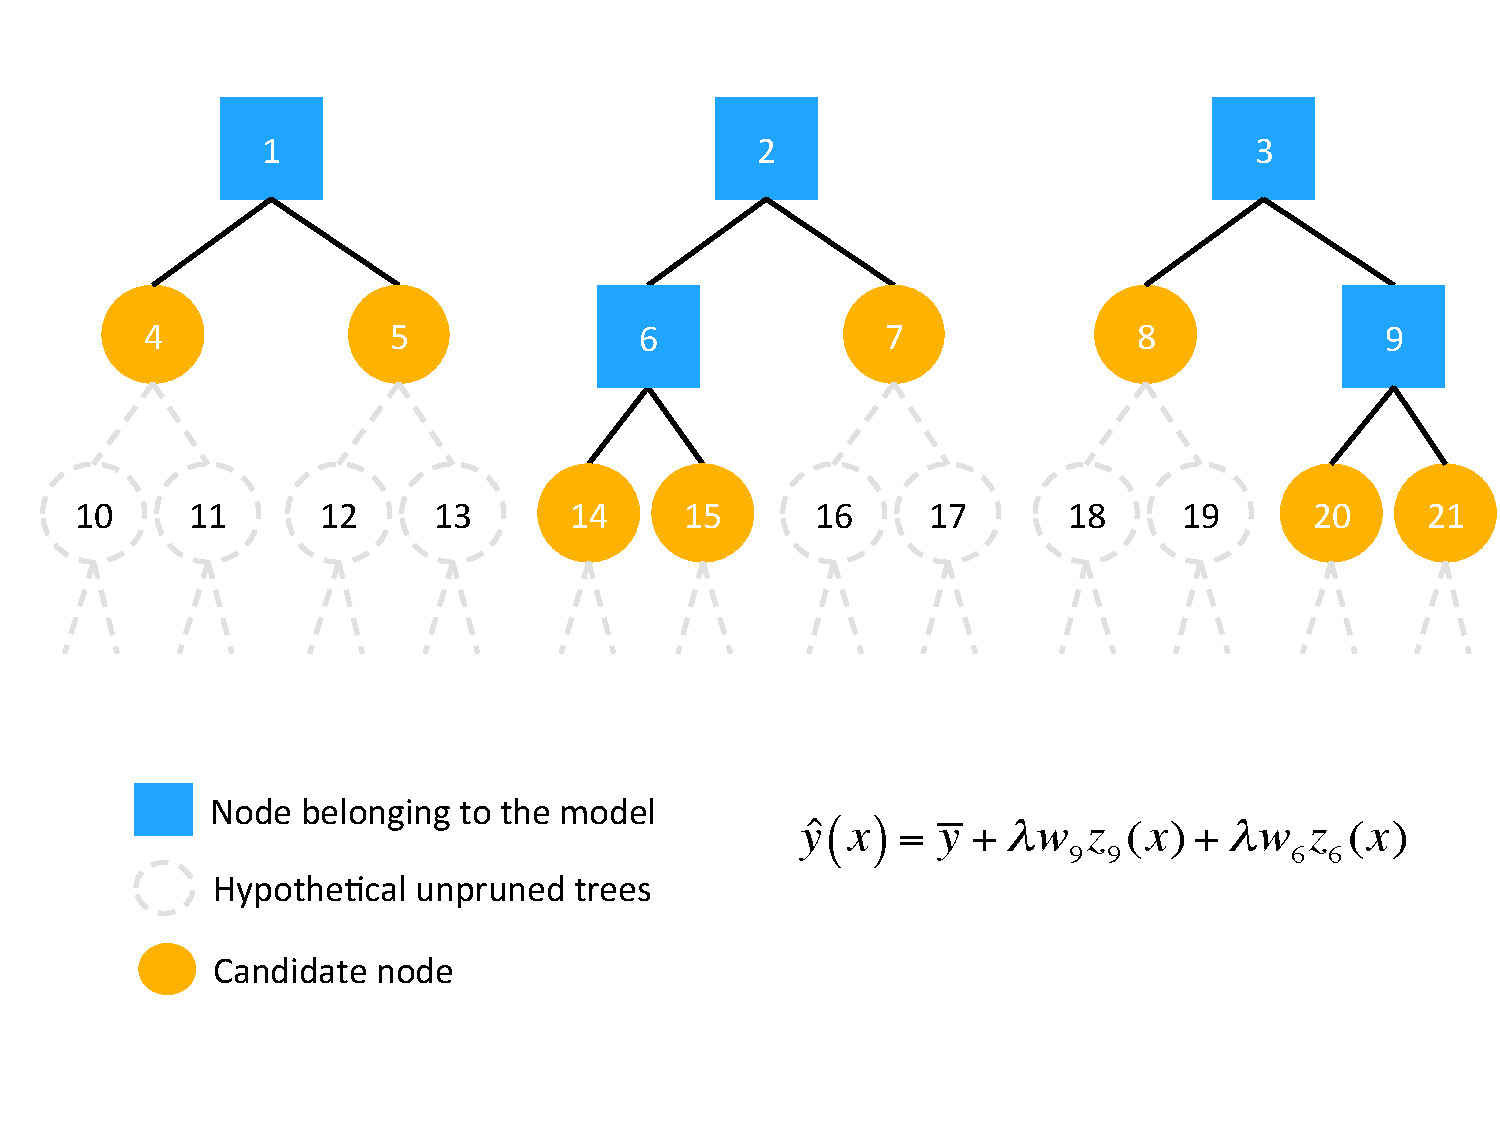
\includegraphics[height=0.25\textheight]{gif_algo6} 
    \caption{The children of the chosen node are computed (step 11) and added 
    to the candidate list (step 12)} 
    \label{fig:gif-algo6} 
  \end{subfigure} 

\caption{Illustration of the GIF regression building algorithm ($T=3$, $CW=3$)}
\label{fig:gif-algo} 
\end{figure*}



\section{Optimization problem}

We are building an additive model by inserting progressively nodes in the 
forest.
At time $t$, we are trying to find the best node $j^{(t)}$ from the candidate 
list $C_t$ and its associated optimal weight $w_j^{(t)}$:
\begin{align}
j^{(t)},w_j^{(t)} =\argmin_{j\in C_t, w\in \mathbb{R}^K} \sum_{i=1}^{N} L 
\left(y_i, 
\hat{y}^{(t-1)}(x_i) + w z_j(x_i) \right)
\end{align}
where $(x_i, y_i)_{i=1}^N$ is the learning sample, $\hat{y}^{(t-1)}()$ is the 
model at time $t-1$, $z_j()$ is the node indicator functions, meaning that it 
is $1$ if its argument reaches node $j$ and $0$ otherwise.

This problem is solved in two steps. First a node $j$ is selected from $C_t$ 
and the corresponding optimal weight, alongside the error reduction, are 
computed. This is repeated for all nodes and the one achieving the best 
improvement is selected.

\paragraph{Regression}
For regression, we used the L2-norm:
\begin{align}
w_j^{(t)} = \argmin_{w\in \mathbb{R}} \sum_{i=1}^{N} L \left(y_i, 
\hat{y}^{(t-1)}(x_i) + w z_j(x_i) \right)^2
\end{align}
and the solution is given by
\begin{align}\label{eq:L2Solution}
w_j^{(t)} = \frac{1}{|Z_j|} \sum_{i \in Z_j} r_i^{(t-1)}
\end{align}
where $r_i^{(t-1)} = y_i - \hat{y}^{(t-1)}(x_i)$ is the residual at time $t-1$ 
for the $i$th training instance and $Z_j = \{1 \leq i \leq N | z_j(x_i)=1\}$ is 
the subset of instances reaching node $j$.

\paragraph{Classification}
For classification we used the multi-exponential loss 
\cite{zhu2009multiadaboost}. First, we need to encode the labels so that
\begin{align}\label{eq:MEencode}
y_i^{(k)} = \begin{cases}
1, &\text{ if the class of } y_i \text{ is } k \\
-\frac{1}{K-1}, &\text{otherwise}
\end{cases}
\end{align}
where $K$ is the number of classes. Notice that $\sum_{k=1}^{K} y_i^{(k)} = 0$.
The optimization then becomes
\begin{align}\label{eq:MEmin}
w_j^{(t)} &=  \argmin_{w \in \mathbb{R}^K} \sum_{i=1}^N \exp 
\left(\frac{-1}{K} y_i^T \left(\hat{y}^{(t-1)}(x_i) + w z_j(x_i) \right)\right) 
\\
&= \argmin_{w \in \mathbb{R}^K} F_j^{(t-1)}(w)
\end{align}
Solving for $\nabla F_j^{(t-1)}(w) = 0$ yields
\begin{align}\label{eq:MErawSol}
\alpha_j^{(t-1, k)}\phi^{(k)}(w) = \frac{1}{K} \sum_{l=1}^{K} \alpha_j^{(t-1, 
l)}\phi^{(l)}(w)
\end{align}
for $1 \leq k\leq K$, where
\begin{align}
\alpha_j^{(t-1, k)} &\triangleq \sum_{i \in Z_j^{(k)}} \exp \left( - 
\mu_i^{(t-1)} \right) \\
\mu_i^{(t-1)} &\triangleq \frac{1}{K} \sum_{k=1}^{K} y_i \hat{y}^{(t-1, 
k)}(x_i) \\
\phi^{(k)}(w) &\triangleq \exp \left( - \frac{1}{K} \psi^{(k)}(w) \right) \\
\psi^{(k)}(w) &\triangleq -w^{(k)} + \frac{1}{K-1} \sum_{l=1, l\neq k}^{K}  
w^{(l)}
\end{align}
where $Z_j^{(k)} = \{1 \leq i \leq N | z_{i,j} = 1 \wedge y_i^{(k)} = 1 \}$ is 
the subset of learning instances of class $k$ reaching node $j$. In words, 
$\mu_i^{(t-1)}$ is the hyper-margin of instance $i$ at time $t-1$ and 
$\alpha_j^{(t-1, k)}$ is the class error of label $k$ for node $j$ at time 
$t-1$.


Equation \ref{eq:MErawSol} is equivalent to
\begin{align}\label{eq:MEequation}
\alpha_j^{(t-1, k)}\phi^{(k)}(w) &= \alpha_j^{(t-1, l)}\phi^{(l)}(w) \quad 1 
\leq k,l \leq K
\end{align}


In keeping with the output representation (Equation \ref{eq:MEencode}), we can 
impose a zero-sum constraint on the prediction to get a unique solution for the 
$k$th component of $w_j^{(t)}$. If it is imposed at each stage, it means that
\begin{align}\label{eq:MEzeroSum}
\sum_{k=1}^{K} \hat{y}^{(t-1, k)} = \sum_{k=1}^{K} 
\hat{y}^{(t, k)} = 0 = \sum_{k=1}^{K} w^{(k)}
\end{align}
and this is not impacted by the learning rate. 

The corresponding solution is
\begin{align}
\phi^{(k)}(w) &= \exp \left(-\frac{1}{K-1} w^{(k)}\right)\\ 
\label{eq:MEClsErrZS}
\alpha_j^{(t-1, k)} &= \sum_{i \in Z_j^{(k)}} \exp \left( -\frac{1}{K-1} 
\hat{y}^{(t-1, k)}(x_i) \right) \\ \label{eq:MEsolution}
w_j^{(t,k)} &= \frac{K-1}{K}  \sum_{l=1}^{K} \log \frac{\alpha_j^{(t-1, 
k)}}{\alpha_j^{(t-1, l)}} 
\end{align}









\section{Equivalence of GIF and the underlying tree}\label{app:Equiv}
In the case of a single tree ($T=1$) and a unit learning rate ($\lambda=1$), 
both the square loss in regression and the multiexponential loss in 
classification produce the same predictions as the underlying tree. 
This is due to the fact that, when examining the weight to give to node $j$ at 
time $t$, the prediction of time $t-1$ relates to the parent node $\pi_j$ of 
$j$. It is thus independent of $t$ and is also the same for all instances 
reaching that node. 

Consequently, we will adopt the following slight change in notation:
\begin{align}
\hat{y}_j = \hat{y}_{(\pi_j)} + w_j
\end{align}
meaning that the prediction associated to any object reaching node $j$ is the 
weight of $j$ plus the prediction associated to its parent $\pi_j$. With  
$\hat{y}_{(\pi_1)} = 0$, the prediction of the root's pseudo-parent.

\subsection{Regression}
In regression, the tree prediction $Tr_j$ of any leaf $j$ is the average of the 
learning set's outputs reaching that node: $Tr_j = \frac{1}{|Z_j|}\sum_{i \in 
Z_j} y_i$. We need to show that the GIF prediction is:
\begin{align}\label{eq:EquivL2Cond}
\hat{y}_{j} = \frac{1}{|Z_j|}\sum_{i \in Z_j} y_i
\end{align}



The prediction of node $j$ is
\begin{align}\label{eq:EquivL2Solution}
\hat{y}_j &= \hat{y}_{\pi_j} + w_j \\
&= \hat{y}_{\pi_j} +  \frac{1}{|Z_j|} \sum_{i \in Z_j} \left(y_i - 
\hat{y}_{\pi_j}\right) \\
&= \hat{y}_{\pi_j} + \frac{1}{|Z_j|} \sum_{i \in Z_j} \left( y_i \right) - 
\hat{y}_{\pi_j} \\
&= \frac{1}{|Z_j|} \sum_{i \in Z_j}  y_i 
\end{align}


The first step is how the additive model is built. The second is the optimal 
weight value of node $j$ derived in Equation \ref{eq:L2Solution}, the third 
step is due to the fact that the prediction at $\pi_j$ is constant since there 
is only one tree.

\subsection{Classification}
In order to have the same prediction as the underlying tree, we must 
demonstrate that the probability of being in class $l$ associated to node $j$ 
will be $\frac{|Z_j^{(l)}|}{|Z_j|}$.

Under the zero-sum constraint, we have
\begin{align} 
\exp \left(  \frac{1}{K-1} w_j^{(l)}\right) &= \frac{1}{c_j} 
\alpha_{\pi_j}^{(l)} \\
&=  \frac{1}{c_j} \sum_{i \in Z_j^{(l)}} \exp \left(-\frac{1}{K-1} 
\hat{y}_{\pi_j}^{(l)}\right)\\
&= \frac{1}{c_j} |Z_j^{(l)}| \exp \left(-\frac{1}{K-1} 
\hat{y}_{\pi_j}^{(l)}\right) \\
\exp \left(\frac{1}{K-1} \hat{y}_j^{(l)} \right) &= \exp \left(\frac{1}{K-1} 
\hat{y}_{\pi_j}^{(l)} \right) \exp \left(\frac{1}{K-1} w_j^{(l)}\right) \\
&= \frac{1}{c_j} |Z_j^{(l)}| \\
P_j(l) &= \frac{\exp \left(\frac{1}{K-1} \hat{y}_j^{(l)}
\right)}{\sum_{k=1}^K\exp \left(\frac{1}{K-1} \hat{y}_j^{(k)} \right)} = 
\frac{|Z_j^{(l)}|}{|Z_j|}
\end{align}	
where $c_j = \left(\prod_{k=1}^K \alpha_j^{(k)}\right)^{\frac{1}{K}}$ is a 
constant. The first equality is a consequence of the value of $w_j^{(l)}$ 
(Equation \ref{eq:MEsolution}). The second is a due to the definition of 
$\alpha_j^{(l)}$ (Equation \ref{eq:MEClsErrZS}). The third is a consequence of 
having a single tree: the prediction of the parent is the same for all 
instances.


Notice that, in both regression and classification, the equivalence also holds 
for an internal node: the prediction is the one the tree would have yielded if 
that node had been a leaf.


\section{Datasets}

Table \ref{tab:datasets} sums up the main characteristics of the datasets we 
used. Abalone, CT slice, California data housig (Cadata), Musk2, Vowel and 
Letter come from the UCI Machine Learning Repository \cite{uci}. Ringnorm, 
Twonorm and Waveform are described in \cite{breiman1998arcing}. Hwang F5 comes 
from the DELVE repository \footnote{http://www.cs.utoronto.ca/∼delve}.
The noise parameter of the Friedman1 dataset \cite{friedman11991} has 
been set to $1$. Hastie is described in \cite{hastie2009}. Out of the 500 
features of Madelon \cite{guyon2004madelon}, 20 are informative and 50 are 
redundant; the others are noise.
Mnist8vs9 is the Mnist dataset \cite{lecun1998mnist} of which only the $8$ and 
$9$ digits have been kept. Binary versions of the Mnist, Letter and Vowel 
datasets have been created as well by grouping the first half and second half 
classes together.

\begin{table}[th]
\caption{Characteristics of the datasets. $N$ is the learning sample size, TS 
stands for testing set, and $p$ is the number of features.}
\label{tab:datasets}
\begin{center}
\begin{footnotesize}
\begin{sc}
\begin{tabular}{l|cccc}
\hline
Dataset & $N$ & $|TS|$ & $p$ & \# classes\\
\hline
Friedman1 & 300 & 2000 & 10 & - \\
Abalone & 2506 & 1671 & 10 & - \\
CT slice & 2000 & 51500 & 385 & - \\
Hwang F5 & 2000 & 11600 & 2 & - \\
Cadata & 12384 & 8256 & 8 & - \\
Ringnorm & 300 & 7100 & 20 & 2 \\
Twonorm & 300 & 7100 & 10 & 2 \\
Hastie & 2000 & 10000 & 10 & 2 \\
Musk2 & 2000 & 4598 & 166 & 2 \\
Madelon & 2200 & 2200 & 500 & 2 \\
Mnist8vs9 & 11800 & 1983 & 784 & 2 \\
Waveform & 3500 & 1500 & 40 & 3 \\
Vowel & 495 & 495 & 10 & 11 \\
Mnist & 50000 & 10000 & 784 & 10 \\
Letter & 16000 & 4000 & 8 & 26 \\
\hline
\end{tabular}
\end{sc}
\end{footnotesize}
\end{center}
\vskip -0.2in
\end{table}

\section{Comparison with local baseline algorithms}
We have tested three deepening algorithm for decision forest relying on 
non-global metrics, meaning that the choice of the best candidate is not made 
according to how well the forest, as a whole, performs. These algorithms share 
that the final model is exactly a sub-forest of the un-pruned forest: contrary 
to GIF, no internal weights are fitted and the prediction of at the leaves are 
the usual tree prediction.

\paragraph{Breadth first deepening}
This variant consist in adding the nodes level after level, from left to right, 
producing a heaped forest. As a consequence, all trees have the same (order of) 
height, implying that the forest can be quite wide but usually shallow.

\paragraph{Random deepening}
This variant consist in first choosing a tree and then choosing one of its 
leaves to transform to a decision nodes. Both choices are made uniformly at 
random so that the trees are expected to have approximately the same number of 
nodes. The depth, however, might vary significantly.

\paragraph{Best first deepening}
This variant consist in choosing, among all leaves which could be turn into a 
internal node, the one which reduces its local impurity the most. Let $I_c$, 
$I_l$ and $I_r$ be the impurity (gini index in classification, variance in 
regression) of the candidate node, candidate left child and candidate right 
child respectively. Let also $N_c$, $N_l$ and $N_r$ be the number of instances 
reaching the candidate node, candidate left child and candidate right child 
respectively. Then, for $N$ learning instances, the local impurity reduction is 
defined as:

\begin{align}
\Delta I_c \triangleq \frac{N_c}{N} \left[ I_c - \left( \frac{N_l}{N_c} I_l + 
\frac{N_r}{N_c} I_r \right)\right]
\end{align}

Since the fraction of learning instances reaching the candidate is accounted 
for in the reduction of impurity, this approach will naturally favor higher 
nodes in the trees.


\begin{table*}[t]
\caption{Average mean square error for local baselines at $1\%$ and $10\%$ 
budgets  ($T=1000$, $m=p$).}
\vskip -0em
\label{tab:baseline-reg}
\begin{center}
\begin{footnotesize}
\begin{sc}
\begin{tabular}{l|ccc|ccc}
\hline
Dataset & Breadth First$_{10\%}$ & Random$_{10\%}$ & Best First$_{10\%}$ & 
Breadth First$_{1\%}$ & Random$_{1\%}$ & Best First$_{1\%}$ \\
\hline
Friedman1 & 6.02 $\pm$ 0.28 & 6.80 $\pm$ 0.34 & 15.00 $\pm$ 0.39 & 11.73 $\pm$ 
0.46 & 12.52 $\pm$ 0.47 & 15.29 $\pm$ 0.42  \\
Abalone & \best 4.72 $\pm$ 0.23 & 4.77 $\pm$ 0.23 & 6.82 $\pm$ 0.33 & 5.42 
$\pm$ 0.27 & 5.55 $\pm$ 0.27 & 6.82 $\pm$ 0.33 \\
CT slice &  30.39 $\pm$ 1.90 & 36.19 $\pm$ 1.84 & 310.87 $\pm$ 4.79 & 82.19 
$\pm$ 2.41 & 97.24 $\pm$ 1.90 & 313.84 $\pm$ 4.64  \\
Hwang F5 \hfill {\tiny $\times 10^{-2}$} & \best 6.73 $\pm$ 0.07 & 6.83 $\pm$ 
0.06 & 56.57 $\pm$ 6.03 & 8.52 $\pm$ 0.24 & 13.17 $\pm$ 0.44 & 56.60 $\pm$ 6.07 
\\
Cadata \hfill {\tiny $\times 10^{-2}$} & 29.24 $\pm$ 0.73 & 31.08 $\pm$ 0.74 & 
75.23 $\pm$ 0.95  & 43.40 $\pm$ 1.18 & 47.47 $\pm$ 1.02 & 75.48 $\pm$ 0.95 \\
\hline
\end{tabular}
\end{sc}
\end{footnotesize}
\end{center}
\vskip -0.2in
\end{table*}


\begin{table*}[t]
\caption{Error rate ($\%$) for local baselines at $1\%$ and $10\%$ budgets 
($T=1000$, $m=\sqrt{p}$). The six firts datasets are binary classification. The 
last three are multiclass. The three in the middle are their binary versions.}
\vskip -1em
\label{tab:baseline-cls}
\begin{center}
\begin{footnotesize}
\begin{sc}
\begin{tabular}{l|ccc|ccc}
\hline
Dataset & Breadth First$_{10\%}$ & Random$_{10\%}$ & Best First$_{10\%}$ & 
Breadth First$_{1\%}$ & Random$_{1\%}$ & Best First$_{1\%}$ \\
\hline 
Ringnorm & 4.25 $\pm$ 1.24 & 4.08 $\pm$ 1.12 & 8.38 $\pm$ 6.94 &  8.94 $\pm$ 
7.45 & 8.53 $\pm$ 7.04 & 8.94 $\pm$ 7.41 \\
Twonorm & 3.51 $\pm$ 0.26 & 3.53 $\pm$ 0.30 & 5.59 $\pm$ 1.85  & 5.91 $\pm$ 
3.03 & 6.52 $\pm$ 4.28 & 7.28 $\pm$ 4.34 \\
Hastie & 11.30 $\pm$ 1.20 & 11.18 $\pm$ 1.16 & 21.24 $\pm$ 7.11  & 13.92 $\pm$ 
2.93 & 14.29 $\pm$ 3.20 & 21.24 $\pm$ 7.12 \\
Musk2 & 7.01 $\pm$ 0.40 & 7.63 $\pm$ 0.43 & 15.42 $\pm$ 0.23 & 15.42 $\pm$ 0.23 
& 15.42 $\pm$ 0.23 & 15.42 $\pm$ 0.23 \\
Madelon & 11.68 $\pm$ 0.67 & 11.92 $\pm$ 0.65 & 19.12 $\pm$ 1.94 & 16.26 $\pm$ 
0.97 & 16.70 $\pm$ 1.07 & 20.14 $\pm$ 2.41 \\
Mnist8vs9 & 2.20 $\pm$ 0.38 & 2.37 $\pm$ 0.39 & 6.17 $\pm$ 0.73  & 4.53 $\pm$ 
0.48 & 4.84 $\pm$ 0.51 & 6.67 $\pm$ 0.69 \\
\hline
Bin. Vowel &8.99 
$\pm$ 1.96 & 8.85 $\pm$ 2.03 & 16.57 $\pm$ 3.02  & 18.73 $\pm$ 3.08 & 19.90 
$\pm$ 3.71 & 21.80 $\pm$ 4.38 \\
Bin. Mnist & 4.46 $\pm$ 0.25 & 4.91 $\pm$ 0.27 & 21.71 $\pm$ 0.30  & 10.09 
$\pm$ 0.25 & 11.78 $\pm$ 0.32 & 22.50 $\pm$ 0.35\\
Bin. Letter & 5.91 $\pm$ 0.43 & 5.71 $\pm$ 0.40 & 26.16 $\pm$ 0.86  & 17.91 
$\pm$ 0.77 & 18.05 $\pm$ 0.78 & 26.19 $\pm$ 0.88 \\
\hline
Waveform & 14.74 $\pm$ 0.63 & 14.83 $\pm$ 0.76 & 20.25 $\pm$ 2.22 & 16.75 $\pm$ 
1.26 & 17.13 $\pm$ 1.25 & 20.45 $\pm$ 2.21 \\
Vowel & 14.26 $\pm$ 2.41 & 13.21 $\pm$ 2.33 & 41.49 $\pm$ 5.45 & 42.40 $\pm$ 
4.33 & 40.28 $\pm$ 4.62 & 50.44 $\pm$ 5.81 \\
Mnist & 4.63 $\pm$ 0.27 & 4.96 $\pm$ 0.26 & 28.54 $\pm$ 0.59 & 8.60 $\pm$ 0.35 
& 9.76 $\pm$ 0.31 & 29.72 $\pm$ 0.61 \\
Letter & 7.06 $\pm$ 0.29 & 6.39 $\pm$ 0.20 & 36.92 $\pm$ 1.80 & 22.11 $\pm$ 
0.59 & 20.90 $\pm$ 0.55 & 37.27 $\pm$ 1.78 \\
\hline
\end{tabular}
\end{sc}
\end{footnotesize}
\end{center}
\vskip -0.2in
\end{table*}

\paragraph{Experiment}
We conducted the same experiment as for GIF: the three algorithms were tested 
on ten folds with different learning sample/testing sample splits and were 
subjected to the $1\%$ and $10\%$ constraints. We started with a pool of 
$T=1000$ roots and no restriction was imposed regarding the depth. All of the 
$m=p$ the features were examined in regression and $m=\sqrt{p}$ in 
classification, as suggested in \cite{extratrees}. Table \ref{tab:baseline-reg} 
holds the average mean square error for the five regression problems and Table 
\ref{tab:baseline-cls} holds the average misclassification rate for the 
classification problems.

\paragraph{Regression}
The trend is quite clear: both at $1\%$ and $10\%$, the breadth first algorithm 
is the best and the best first is (largely) the worst. 
There are two instances where the local baselines are able to beat GIF: on 
Abalone and Hwang F5 at $10\%$. Interestingly, these are the same cases on 
which GIF was beaten by a small forest of Extremely randomized trees. The 
$10\%$ Hwang F5 case aside, the local baselines always underperform the smaller 
fully-developed forest. Overall, such variants do not seem adequate for 
regression.

\paragraph{Classification}
In classification, the breadth first and random baselines tend to perform 
similarly, one beating the other on some problems. Once again, the best first 
approach seems to be lagging behind on some datasets. At $10\%$, the local 
baselines cannot rival with the other methods. Only on Waveform are they able 
to reach the other performances. However, all methods seems to produce close 
results. At $1\%$, the breadth first and/or the random methods surpass the 
ET$_{10\%}$ on Twonorm, Hastie, Madelon and Waveform. Those datasets correspond 
to cases where ET was under-performing significantly compare to GIF. All in 
all, the local baselines are never able to beat GIF, even in the multiclass 
setting, which is particularly defavorable for GIF. Once again, the conclusion 
is against the local baselines.


We believed the poor performances of the baselines are due to the building 
mechanism of traditional ensemble methods. Although the trees are built 
independently and with randomization, there remains an important redundancy 
between them, which is especially defavorable to pruning. A global approach is 
better able to avoid redundancy and can thus better exploits the node budget. 
This would also explain why the best first variant performs worst in both 
regression and classification: it is prone at picking redundant nodes, which 
will usually offer the same kind of impurity reduction.





\bibliography{gif}
\bibliographystyle{icml2017}

\end{document} 

